\begin{frame}{Robustness result: GSM8K vs. GSM-HARD}

\vspace{0.3cm}


\begin{columns}[T,totalwidth=\textwidth]
      \begin{column}{0.45\textwidth}

        \centering
          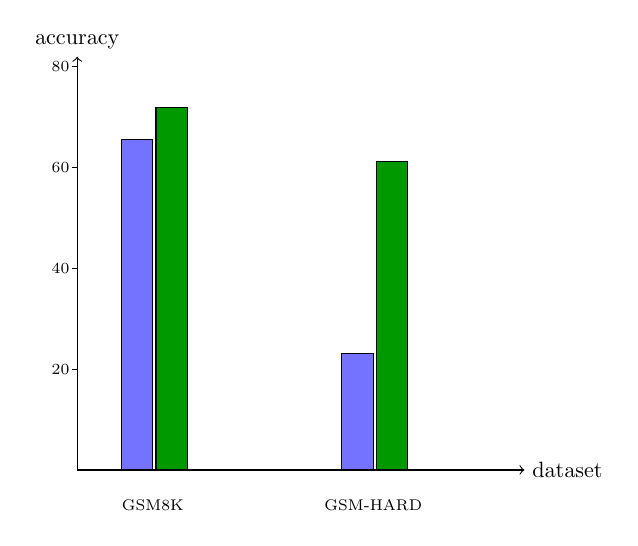
\begin{tikzpicture}[scale=0.8, transform shape, x=1cm,y=0.08cm]
          \draw[->] (0,0) -- (7.1,0) node[right]{dataset};
          \draw[->] (0,0) -- (0,82) node[above]{accuracy};

          \foreach \y in {20,40,60,80}
              \draw (-0.08,\y) -- (0,\y)
              node[left]{\scriptsize \y};

          \node at (1.2,-7) {\scriptsize GSM8K};
          \node at (4.7,-7) {\scriptsize GSM-HARD};

          \draw[fill=blue!55] (0.7,0) rectangle (1.2,65.6);
          \draw[fill=green!60!black] (1.25,0) rectangle (1.75,72.0);

          \draw[fill=blue!55] (4.2,0) rectangle (4.7,23.1);
          \draw[fill=green!60!black] (4.75,0) rectangle (5.25,61.2);

          \node[blue!55!black] at (6.2,65) {\scriptsize \CoT{}};
          \node[green!40!black] at (6.2,56) {\scriptsize \PAL{}};
          \end{tikzpicture}\\
          \source{PAL paper, Table 1 and Section 5.1.}

      \end{column}

      \begin{column}{0.45\textwidth}
          \begin{block}{GSM-HARD construction}
            The authors create a harder variant of GSM8K by replacing numbers in the questions with larger numbers, including values up to seven digits.
          \end{block}
          \begin{alertblock}{Observed failure mode}
            For many examples, \CoT{} produces nearly the same reasoning text for the original and hard versions, suggesting that the main problem is arithmetic execution rather than decomposition.
          \end{alertblock}
      \end{column}

	
      \end{columns}







\end{frame}
